\section{Project and Timeline Management}

\subsection{Completion Timeline}

The project proceeded in five stages: (1) prototype construction (edge node, server, dashboard); (2) public-dataset probing (Phase~1); (3) calibration analysis (Phase~2); (4) forensic-integrity testing (Phase~3); and (5) the locked baseline comparison (Phase~4, $\approx$ 3.5 hours wall-clock on CPU-only hardware). Each experiment directory records its command, timestamp, git commit, and hardware provenance, providing the audit trail used throughout this book.

\subsection{Gantt Chart}

\begin{figure}[H]
\centering
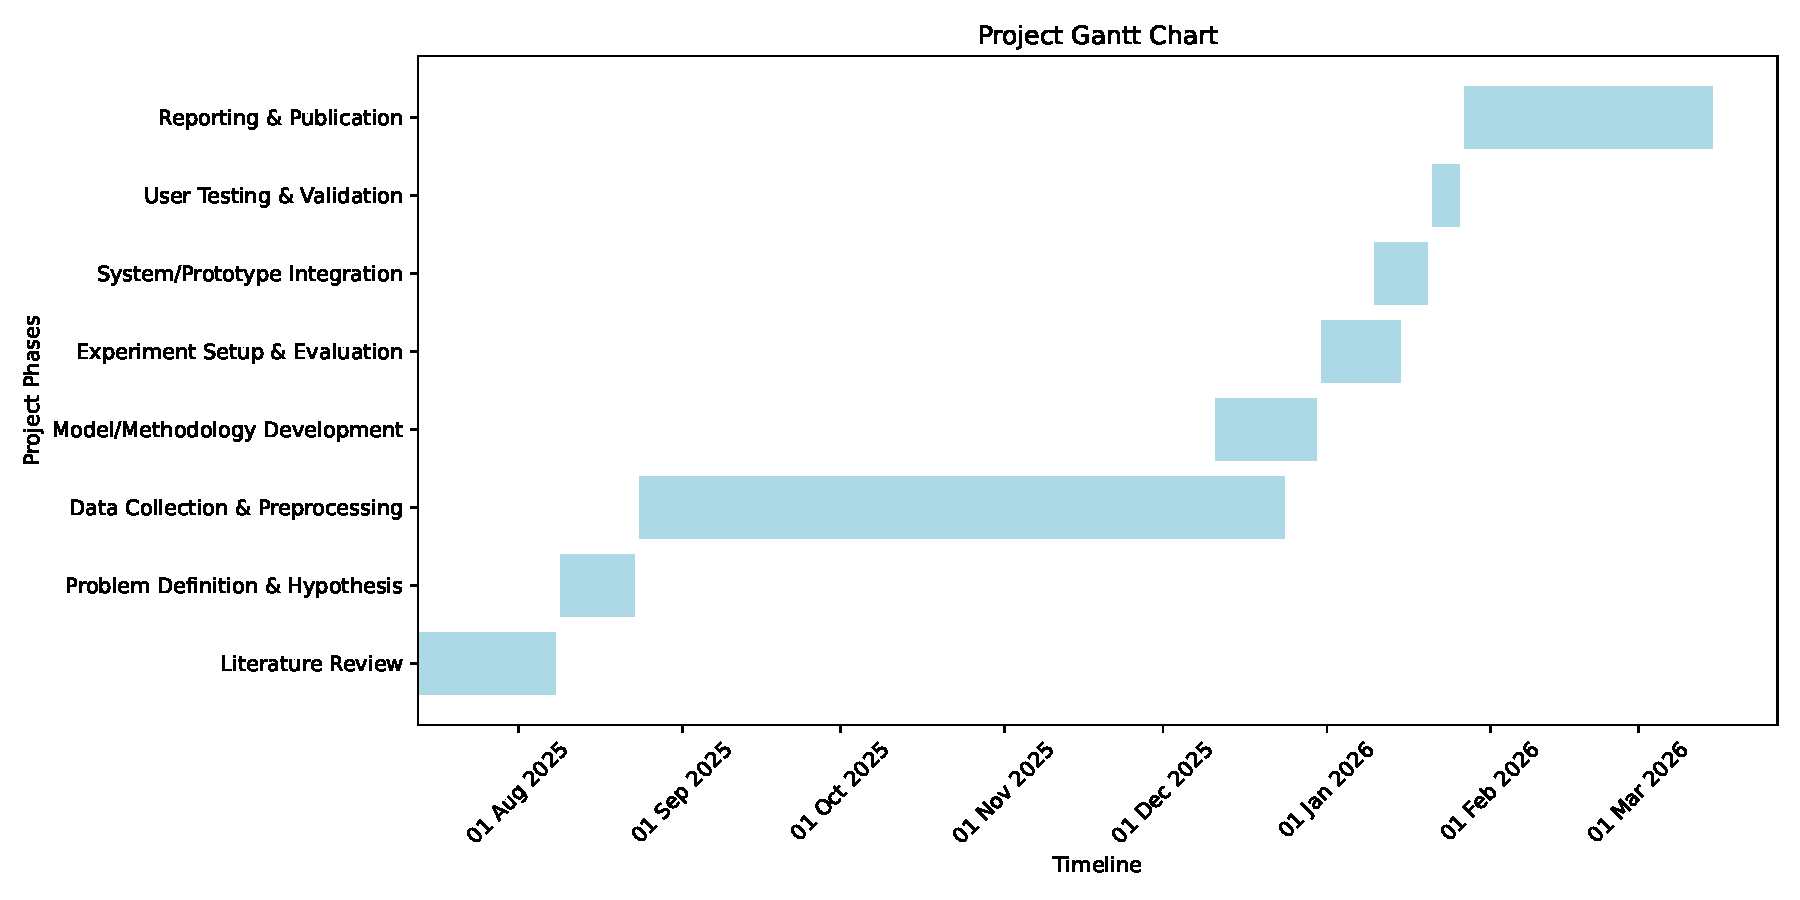
\includegraphics[width=\textwidth]{figures/gantt_chart_lightblue.pdf}
\caption{Gantt Chart of Project Timeline}
\label{fig:gantt-chart}
\end{figure}

\subsection{Financial Statement}

No specialized hardware was procured: all experiments ran on an existing CPU-only machine (Intel i3-6006U, no GPU) with commodity cameras, open-source software (Python, FFmpeg, YOLOv8n weights, Node.js, Next.js), and locally assembled datasets. The project therefore incurred no significant hardware or licensing cost.

\subsubsection{Budget Justification}

The zero-procurement budget is justified by the deployment scenario itself: the system is designed for low-cost, CPU-only operation, so developing and evaluating it on exactly such hardware strengthens rather than weakens the validity of the reported behaviour.
